 \newpage

\subsubsection{XGBoost}
\label{sec:xgboost}

A series of models were trained using an exploratory and iterative approach; RandomizedSearchCV was also utilised in the training phase to optimise hyperparameters. Table \ref{tab:xgboost-parameters} shows the parameters used for each model, \textbf{-} denotes that no value was used, i.e., the default value was used.

\begin{table}[h]
  \centering
  \caption{XGBoost Model Parameters}
  \label{tab:xgboost-parameters}
  \begin{tabular}{lcccccc}
    \toprule
    Parameter & Model 0-2\&6 & Model 3 & Model 5 & Model 8 & Model 10 & Model 11 \\
    \midrule
    early\_stopping\_rounds & - & 10 & 10 & 10 & 10 & 10 \\
    subsample & - & - & - & - & 0.9 & - \\
    n\_estimators & - & - & 300 & 300 & 200 & 300 \\
    min\_child\_weight & - & - & - & - & 3 & - \\
    max\_depth & - & - & 5 & 5 & 9 & 5 \\
    learning\_rate & - & - & 0.2 & 0.2 & 0.3 & 0.2 \\
    gamma & - & - & - & - & 0 & - \\
    colsample\_bytree & - & - & - & - & 0.7 & - \\
    reg\_alpha & - & 0.1 & 0.1 & 0.1 & - & 0.1 \\
    \bottomrule
  \end{tabular}
\end{table}


\medskip

Initial experimentation began with the XGBoost classifier being trained with default parameters across a range of subsets of data, 60\%, 80\% and 100\% as shown in models 0, 1 and 6. Additionally, model 1 further incorporated Stratified Cross Validation during training. This was used to establish clear baseline performance of the classifiers and helped to provide context when tuning parameters.

Where available, the VM machine was used for training, allowing XGBoost to maximise its performance on the dedicated GPU. Early stopping and regularisation were added in subsequent models to help avoid the model from overfitting on the training data. However, in Model 3, early stopping and regularisation were added, with no noticeable performance increase/decrease observed. 

\subsubsection*{Parameter Tuning}

An attempt was made to utilise GridSearchCV for parameter optimisation; significant setbacks were encountered in achieving a successful execution due to numerous errors, system crashes, and exceptionally high grid search time. In light of the difficulties faced with GridSearchCV, RandomizedSearchCV was utilised. 

Initial experimentation with parameter searching on a smaller grid on the 80\% dataset was successful, and subsequent parameters were tested with models 5 and 8. An additional RandomizedSearchCV was run on the entire dataset and combined with stratified 10-fold cross-validation to ensure the best-found parameters were verified and consistent across the ten folds.

See Listing \ref{lst:param_grid_xgb} for the parameter grids used.

\medskip
	
\begin{lstlisting}[language=Python, caption={Grid Search Parameters For XGBoost}, label= lst:param_grid_xgb]

gscv_param_grid = {
    'learning_rate': [0.05, 0.1, 0.2],
    'n_estimators': [100, 200, 300],
    'max_depth': [3, 4, 5]
}

rgs_param_grid = {
    'learning_rate': [0.01, 0.1, 0.3],
    'max_depth': [3, 6, 9],
    'min_child_weight': [1, 3, 5],
    'gamma': [0, 0.1, 0.2],
    'subsample': [0.5, 0.7, 0.9],
    'colsample_bytree': [0.5, 0.7, 0.9],
    'n_estimators': [100, 200]
}
\end{lstlisting}

\begin{table}[H]
\captionsetup{justification=centering} 
\centering
\caption{XGBoost GridSearch Best Parameters}
\begin{tabular}{lll}
\hline
\textbf{Parameter} & \textbf{GS} & \textbf{RGS} \\ \hline
Early Stopping & - & 10 \\
Evaluation Metric & merror & merror \\
Learning Rate & 0.2 & 0.3 \\
Max Depth & 5 & 9 \\
Min Child Weight & - & 3 \\
Gamma & - & 0 \\
Subsamples & - & 0.9 \\
Colsample By Tree & - & 0.7 \\
N Estimators & 300 &  200 \\ \hline
\end{tabular}
\label{tab:xg_gs_parameters}
\end{table}

\textbf{Best Found Parameters}
\medskip

The parameter tuning process helped to identify a set of optimal parameters using RandomisedSearchCV, as detailed in Table \ref{tab:xg_gs_parameters}. These parameters were used to create Model 10. Subsequent models made afterwards, from additional parameter tuning, did not show a noticeable improvement in the model's performance. Due to limited time and computational power, further parameter tuning was not performed, and the decision was made here to stop further experiments.

\subsubsection{K-Nearest Neighbor}

During initial experimentation, KNN took over 22 hours to predict on the test set following training - Figure \ref{fig:knn_train}. Additionally, utilising the VM machine to train, KNN took over 28 hours to predict the data test set and crashed the system multiple times before results or evidence could be gathered. KNN's algorithm means it does not build and store a model during training but keeps them in memory. As a result, predicting on the test set required high computational power as KNN searches for the K-nearest neighbour from the training set. Due to a large number of features, this further increases the computational power required for these tasks. This was deemed too long for real-world applications where detecting network attacks would be time-sensitive. As network attacks can occur quickly, an IDS using ML algorithms needs a quick response to detect these attacks.

Therefore, despite the advantages of KNN, such as being easy to implement and interpret, the prioritisation of speed and accuracy in this work led to the ultimate decision not to continue with this classifier. Consequently, the results for this classifier remain inconclusive.

\medskip

\begin{figure}[h]
\caption{Training Time for KNN Classifier}
\label{fig:knn_train}
\centering
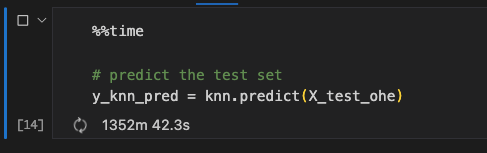
\includegraphics[width=\textwidth]{Appendices/Images/knn_predict-2023-04-15.png}
\end{figure}